\section{A Lifecycle Framework for Computer-Use Agents: From Capability Formation to Continual Adaptation}
\label{sec:lifecycle}

If Section~\ref{sec:architecture} explains what a CUA is made of internally, this section asks how those capabilities become operative in a real system. The comparative point of the lifecycle view is that similar runtime failures may reflect very different upstream causes, and similar design choices may become safe or unsafe depending on when they are introduced. More precisely, the tri-layer architecture offers a structural account of capability composition, whereas the lifecycle perspective explains how perceptual grounding, decision-making, and action execution are produced, bound to concrete platforms, stressed during use, and revised over time. The two views are therefore complementary: the architectural framework clarifies internal organization, while the lifecycle framework clarifies how that organization becomes a functioning, deployable, and governable agent in practice.

To capture this temporal and engineering dimension, we organize representative CUA research into four stages: \textit{Creation}, \textit{Deployment}, \textit{Operation}, and \textit{Maintenance}. This categorization should not be understood as a purely chronological decomposition of system development. Rather, it is motivated by a different analytical question: \emph{at what point in the lifecycle are capabilities formed, operationalized, stressed, and revised?} From this perspective, each stage identifies a distinct locus of capability formation, failure exposure, and safety intervention. Creation determines what perceptual and control priors an agent can acquire through data, model design, and training; Deployment governs how those capabilities are bound to interfaces, tools, permissions, and middleware; Operation tests whether the agent can sustain coherent behavior over long trajectories in open-ended environments; and Maintenance addresses whether the system remains reliable as interfaces drift, workflows change, and adversarial surfaces evolve. Although these stages are tightly coupled in practice and often iterated rather than traversed only once, they capture the dominant points at which CUA capability and risk are shaped across the full system lifecycle.

This shift matters analytically. Many failures that become visible during operation are rooted earlier in the lifecycle---for example, in the quality of grounding established during Creation or in the action abstractions and trust boundaries introduced during Deployment. Conversely, many apparent capability improvements matter only if they survive long-horizon operation and remain stable under post-deployment change. A lifecycle framework therefore does more than reorder prior work: it reveals where bottlenecks originate, where risks surface, and where evaluation and governance must intervene across the full trajectory of a deployed CUA.

\begin{figure*}[t]
\centering
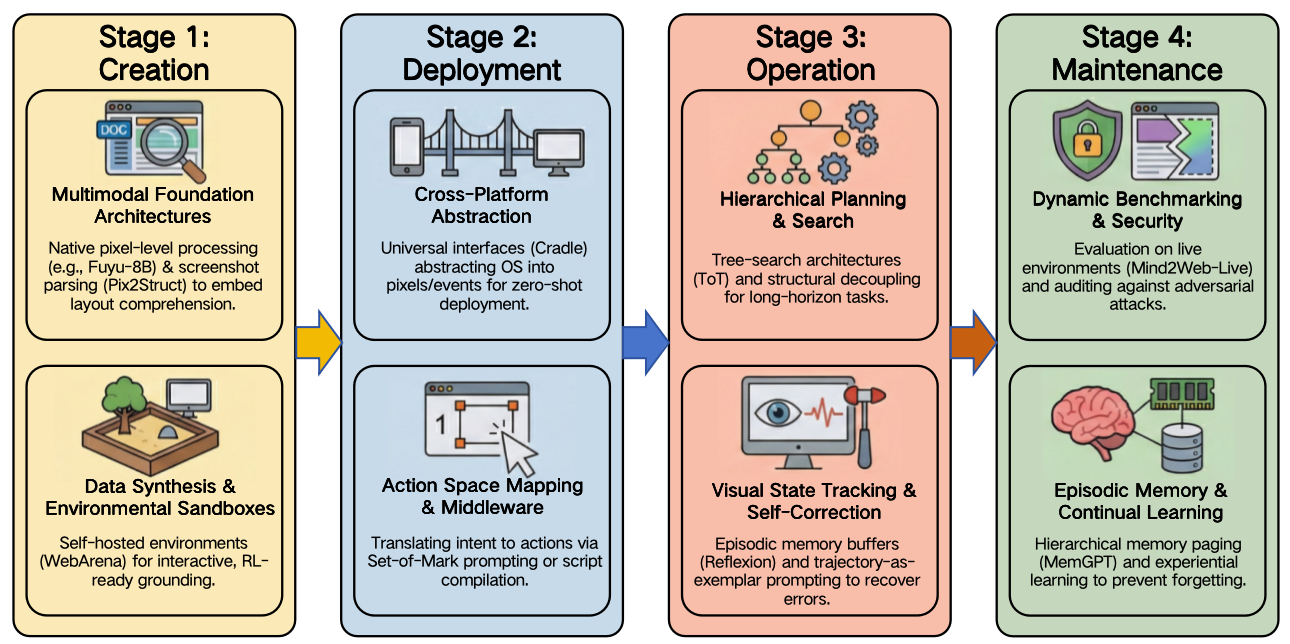
\includegraphics[width=\textwidth]{images/p4.1.png}
\caption{Four-stage lifecycle framework for CUAs: Creation, Deployment, Operation, and Maintenance. The stages correspond to capability formation, system binding, online stress, and continual adaptation.}
\label{fig:lifecycle_taxonomy}
\end{figure*}

\subsection{Creation Stage: Capability Formation Through Grounding, Data, and Training}

The Creation stage determines the \emph{capability ceiling} of a CUA before it interacts with a live environment. The key judgment in this stage is that many later robustness problems are not primarily runtime reasoning failures; they are inherited from what the system was taught to perceive, predict, and optimize. Its goal is not simply to scale model size, but to align \emph{semantic intent}, \emph{visual grounding}, and \emph{actionable interface structure} in ways that support downstream control. This stage is therefore most closely tied to the \emph{Perception Layer}: whether an agent can robustly interpret screens, localize interface elements, and distinguish task-relevant affordances is largely determined here.

Conceptually, Creation is analytically distinct because it is the stage at which usable control priors are \emph{acquired} rather than merely exercised. Accordingly, the most informative way to organize work at this stage is by the mechanisms through which actionable grounding is built: multimodal representation learning, trajectory and reward construction, and interactive training environments. These directions are not entirely separable in mature systems, but together they define the main routes through which pre-deployment capability is formed.

\paragraph{Multimodal grounding as the core bottleneck}
Earlier web agents relied heavily on structured states such as DOM trees, with methods like Mind2Web highlighting the need for filtering and task-centric distillation when raw interface representations become too large or noisy~\cite{deng2023mind2web}. Recent CUA research, however, increasingly treats GUI grounding as a first-class problem in its own right. CogAgent \cite{hong2024cogagent}, ScreenAI \cite{baechler2024screenai}, and SeeClick \cite{cheng2024seeclick} improved visual understanding and point-level action grounding, while newer systems such as WinClick \cite{hui2025winclick} show that pure screenshot-based grounding on desktop environments remains difficult without dedicated pretraining and benchmark design. The broader lesson is that creation-stage progress is no longer just about better multimodal encoders; it is about learning a stable mapping from heterogeneous visual interfaces to executable action semantics.

\paragraph{Data generation, reward design, and interactive training environments}
Recent work also shows that model quality is inseparable from the quality of trajectories, rewards, and environments used to train it. Classical datasets such as AITW \cite{rawles2023androidinthewild} and agent-tuning pipelines such as AgentTuning \cite{zeng2024agenttuning} established the importance of instruction-following trajectories, but they are increasingly complemented by more scalable and adaptive data sources. Open-foundation efforts such as OpenCUA \cite{wang2025opencua} extend this logic with large-scale demonstration capture, cross-OS task coverage, and end-to-end open CUA models. TongUI \cite{zhang2025tongui}, for example, converts multimodal web tutorials into large-scale GUI trajectories across platforms, while UI-R1 \cite{lu2025ui} and GUI-R1 \cite{luo2025gui} demonstrate that reinforcement learning with explicit action rewards can improve action prediction and generalization beyond pure supervised fine-tuning. Meanwhile, interactive environments such as WebArena \cite{zhou2023webarena} and OSWorld \cite{xie2024osworld} remain essential because they expose agents to non-stationary transitions, delayed consequences, and recovery behavior that static corpora cannot faithfully represent.

Overall, the Creation stage defines whether a CUA merely recognizes interface tokens or genuinely acquires \emph{actionable grounding}. It therefore sets the upper bound for downstream robustness. Many errors that later appear during operation---such as unstable localization, failure under visual ambiguity, or brittle transfer to unseen applications---often reflect representational or data limitations introduced at this stage rather than purely online reasoning failures.

\subsection{Deployment Stage: Binding Model Capability to Real Systems}
\label{sec:deployment}

If the Creation stage determines what a model can potentially understand, the Deployment stage determines how that capability is \emph{bound} to a real computing environment. The central comparative claim here is that deployment is where capability turns into authority, and it is often the stage that most directly sets the eventual blast radius of failure. This stage moves the problem from model construction to interface integration: observations must be attached to concrete platforms, and abstract action intent must be translated into executable control channels. Deployment is therefore not a passive implementation detail; it is where capability meets operating-system constraints, middleware, permissions, and platform heterogeneity.

Deployment forms a separate analytical stage because a capable model does not automatically become a usable agent. Between learned capability and real-world operation lies a system-binding problem: what interface is exposed, what actions are permitted, what middleware mediates intent, and what trust boundary surrounds execution. This is increasingly evident in open deployment systems illustrated by \textbf{OpenClaw}, whose public descriptions suggest a continuously reachable gateway that connects messaging channels, sessions, tools, and execution events into a shared control plane. In such systems, deployment is no longer merely a wrapper around a model; it is the stage at which user-facing communication surfaces, execution authority, and policy constraints are assembled into an operational agent stack.

For this reason, deployment work is most naturally organized by how it resolves the tension between broad portability and controlled actuation. In current CUA systems, this tension is most visible in two recurring design choices: whether to favor universal cross-platform interfaces or tighter environment-specific mediation, and how much semantic abstraction to insert between model output and executable action.

\paragraph{Universal interfaces and cross-platform abstraction}
A major design choice in deployment is whether to rely on platform-specific structure or system-agnostic control. Cradle \cite{tan2024cradle} exemplifies a universal philosophy by using screen pixels as input and keyboard/mouse events as output, enabling operation in visually rich environments without application-specific APIs. Related systems such as Mobile-Agent \cite{wang2024mobile}, OS-Copilot \cite{wu2024copilot}, and ScreenAgent \cite{niu2024screenagent} similarly emphasize broad deployability across mobile, desktop, and remote environments. Recent surveys of GUI and OS agents reinforce that such designs improve portability, but also increase dependence on strong visual grounding and low-level control stability~\cite{tang2025survey,hu2025agents}.

As publicly described, OpenClaw makes this deployment logic especially visible because the system is not tied to a single application surface. Instead, it appears as a multi-channel ingress layer spanning platforms such as WhatsApp, Telegram, Slack, Discord, and iMessage while remaining local-first in its control architecture. This kind of design expands portability in a deployment sense: the same agent can be reached across heterogeneous communication interfaces and remain continuously available beyond the workstation on which it runs. At the same time, it shifts more burden onto deployment-time policy design, since cross-channel exposure broadens the range of untrusted inputs, contextual ambiguity, and authority-routing decisions that the system must mediate.

\paragraph{Action abstraction, middleware, and trust boundaries}
Portability alone, however, does not guarantee reliable execution. A second line of work therefore introduces intermediate abstractions that reduce the gap between language-level intent and environment-level control. WebVoyager \cite{he2024webvoyager} uses Set-of-Mark prompting to simplify visual selection, OmniACT \cite{kapoor2024omniact} compiles decisions into executable scripts, and UFO \cite{zhang2025ufo} separates application selection from local action execution in desktop environments. These systems suggest that deployment success depends not only on \emph{where} an agent is mounted, but also on \emph{how} semantic intent is mediated before emission as low-level actions.

Deployment is also the stage where trust boundaries become concrete. In OpenClaw-like deployments, operators must make explicit decisions about which channels may reach the agent, which tools are enabled, whether sandboxing is applied, how sessions are isolated, and how network and automation settings are configured. These choices determine whether middleware acts as a safety-enforcing constraint layer or merely as a conduit for unconstrained execution. More broadly, deployment-time abstractions can either reduce downstream risk by narrowing action pathways and scoping authority, or amplify it by centralizing control while leaving permissions, extension points, and execution surfaces insufficiently separated.

Taken together, the Deployment stage is defined by a central trade-off between \emph{portability} and \emph{controllability}. System-agnostic interfaces generalize broadly, but they place heavier burdens on grounding and verification. More tightly integrated middleware can improve determinism and efficiency, but it introduces stronger assumptions about privileges, dependencies, and trusted execution channels. Publicly described open-deployment systems such as OpenClaw make this trade-off especially salient: once communication channels, tool invocation, session state, and system execution are bound through a single gateway layer, many failures that later appear as ``agent mistakes'' are in fact rooted in deployment-time decisions about abstraction, authority, and trust boundaries.
\subsection{Operation Stage: Long-Horizon Interaction, Memory, and Recovery}
\label{sec:operation}

Once deployed, a CUA enters the stage where its practical value is actually tested: live operation under changing interface states and real tasks. The main comparative result at this stage is that long-horizon reliability depends less on single-step plausibility than on memory discipline, verification, and recovery. At this point, the main challenge is no longer whether the agent can parse a screen or emit an action in principle, but whether it can maintain task coherence across long trajectories without drifting, looping, or compounding local mistakes. Accordingly, the Operation stage is where the \emph{Decision Layer} faces its greatest pressure.

Operation is analytically distinct because it is the point at which latent capability is exposed to real temporal stress. In this stage, failures are no longer hypothetical limitations of representation or interface binding; they become observable breakdowns in continuity, recovery, and control under non-stationary interaction. For this reason, the main axes of progress are best understood in terms of how systems sustain coherence online: by adding stronger execution structure, by preserving memory across steps, and by verifying whether previous actions actually produced the intended state changes.

\paragraph{From step-wise reaction to structured execution}
Earlier agent frameworks such as ReAct \cite{yao2022react} and Tree of Thoughts \cite{yao2023tree} established the value of explicit reasoning and search. In the CUA setting, however, recent work shows that planning must be combined with stronger execution structure. MobileUse \cite{li2025mobileuse} introduces hierarchical reflection to detect and recover from failures at multiple temporal scales, while WorldGUI \cite{zhao2025worldgui} demonstrates that current GUI agents degrade sharply under diverse initial states, revealing fragile long-horizon planning even when single-step actions appear plausible. ActionEngine \cite{zhong2026actionengine} pushes this trend further by shifting from reactive control toward programmatic execution based on an updatable GUI state-machine memory. Recent scaling results reinforce the same lesson from a different angle: Behavior Best-of-N improves OSWorld performance and generalizes to WindowsAgentArena and AndroidWorld by selecting among multiple rollouts through structured behavior narratives, suggesting that operational reliability depends on trajectory selection and verification rather than one-shot planning alone~\cite{gonzalez2025scalingcua}.

\paragraph{Memory, verification, and fault tolerance}
Recent literature also makes clear that long-horizon success depends not only on planning, but on runtime memory and post-action verification. Reflexion \cite{shinn2023reflexion} and Synapse \cite{zheng2023synapse} already suggested that agents benefit from self-feedback and experience reuse. More recent GUI-specific work sharpens this observation: execution failures increasingly stem from state loss, weak memory across steps, and the inability to verify whether prior actions had the intended effects. This is precisely why contemporary CUA research is moving toward structured memory, reflective recovery, and verifier-driven control rather than relying on a single monolithic prompt.

OpenClaw-like systems make this pressure especially concrete because persistent messaging channels and long-lived sessions compress multiple tasks, users, and contextual cues into the same runtime surface. In such deployments, weak memory scoping or inadequate post-action verification does not merely reduce benchmark accuracy; it can allow stale context, cross-task contamination, or ambiguous channel intent to persist across operational episodes.

The Operation stage is where local mistakes become global failures unless they are actively contained. Better planning, memory, and verification generally improve long-horizon robustness, but they also increase latency, context cost, and system complexity. The key challenge is therefore not merely to make agents more autonomous, but to make that autonomy \emph{stable} under environmental non-stationarity.

\subsection{Maintenance Stage: Continual Adaptation, Evaluation, and Security Hardening}
\label{sec:maintenance}

Unlike static benchmark models, CUAs operate in software ecosystems that evolve continuously. The main comparative lesson of the Maintenance stage is that post-release stability is itself an engineering variable: a strong system can decay quickly if evaluation, permissions, and ecosystem controls remain frozen while the environment changes. Interfaces are redesigned, workflows shift, permissions change, and adversarial surfaces emerge after deployment. For this reason, Maintenance should not be understood as a final cleanup stage after operation; it is the \emph{continual adaptation layer} that keeps the entire system valid over time.

Maintenance is best treated as a distinct stage because post-deployment validity is not guaranteed by one-time success at deployment or operation. Even a well-trained and initially well-behaved agent will degrade if the surrounding software ecosystem changes while its assumptions remain fixed. The core question of this stage is therefore how to preserve reliability under drift, shifting workflows, stale evaluation signals, and evolving attack surfaces. From this perspective, recent work can be read through three recurring maintenance functions: adaptation to interface and workflow change, continuous reliability evaluation, and post-deployment security hardening.

\paragraph{Adapting to UI drift and workflow change}
A first maintenance challenge is preserving capability under changing interfaces. Recent work shows that GUI failure is often caused not by complete task novelty, but by gradual visual and procedural drift. MAGNET \cite{sun2026magnet}, for example, explicitly addresses appearance drift and workflow drift through dual-level memory that separates stable functional semantics from evolving task procedures. This reframes maintenance as an ongoing problem of retaining invariant knowledge while updating interface-specific realizations.

\paragraph{Continuous evaluation and memory-aware reliability testing}
A second challenge is that static benchmarks quickly become stale in GUI environments. VisualWebArena \cite{koh2024visualwebarena}, WorkArena \cite{drouin2024workarena}, and Risky-Bench \cite{zheng2026riskybench} already move evaluation closer to realistic web, enterprise, and deployment-grounded settings, but recent evidence suggests that even these are not sufficient to characterize long-term reliability. MemGUI-Bench \cite{liu2026memgui} shows that existing mobile GUI benchmarks severely under-represent memory-intensive tasks and fail to assess cross-session learning, implying that maintenance requires continuous, capability-targeted evaluation rather than one-time benchmark success.

\paragraph{Security as a lifecycle maintenance problem}
Finally, maintenance must include post-deployment security hardening. Zero-Permission Manipulation \cite{qian2026zero} shows that GUI agents can be exploited through the observation-to-action gap, allowing malicious interfaces to rebind seemingly benign planned actions without requiring dangerous permissions. More recent deployment-facing studies make the same point in broader form: PASB \cite{wang2026pasb} reports vulnerabilities across prompt processing, tool usage, and memory retrieval in personalized OpenClaw scenarios, while Your Agent, Their Asset \cite{wang2026asset} shows that poisoning persistent capability, identity, or knowledge state can sharply raise attack success rates. ClawKeeper \cite{liu2026clawkeeper} responds with skill-, plugin-, and watcher-based protections intended to span multiple lifecycle stages. Together, these results suggest that some safety failures are not caused by poor reasoning alone, but by architectural assumptions that only become visible after deployment in dynamic environments. Maintenance must therefore include regression testing, attack-surface monitoring, and policy updates alongside model adaptation.

The same point extends to open ecosystems illustrated by public discussions around OpenClaw and Moltbook. Once tools, channel integrations, or agent communities evolve independently of the base model, maintenance must govern not only model quality but also ecosystem hygiene: version pinning, extension review, identity management, and policies for capability sharing become part of the reliability problem rather than optional platform administration~\cite{wang2026asset,liu2026clawkeeper}.

Taken together, the Maintenance stage reveals a final trade-off: continual updating improves adaptation and resilience, but it also increases evaluation overhead, regression risk, and governance complexity. Conversely, freezing a deployed system may preserve short-term stability, yet it leads to rapid decay once interfaces, workflows, or threat models change. For CUAs, maintenance is therefore not the last step in a linear pipeline; it is the mechanism that keeps the whole lifecycle operational.

\begin{table*}[!t]
\centering
\scriptsize
\caption{Illustrative mapping of OpenClaw-related deployment properties onto the master framework.}
\label{tab:openclaw_mapping}
\renewcommand{\arraystretch}{1.08}
\setlength{\tabcolsep}{3.5pt}
\begin{tabularx}{\textwidth}{L{2.75cm} L{1.8cm} L{2.8cm} Y}
\toprule
\textbf{Property} & \textbf{Location} & \textbf{Risk} & \textbf{Control} \\
\midrule
Persistent messaging ingress across channels~\cite{openclaw2026website,ibm2026openclaw} & Deployment & Mixed trust levels, ambiguous sender intent, broad ingress & Channel isolation, provenance tagging, session scoping \\
Local-first control plane bound to tools and sessions~\cite{openclaw2026website} & Deploy. + oper. & Concentrated authority, over-privilege, weak mediation & Least privilege, sandboxing, auditable mediation, approval for high-impact actions \\
Persistent sessions and carried-over runtime context & Operation & Cross-task contamination, stale context, verifier failure & Memory partitioning, expiry/reset policy, post-action verification \\
Agent-community or Moltbook-style capability exchange~\cite{chen2026openclaw} & Oper. + maint. & Capability diffusion, prompt propagation, ecosystem exposure & Signed exchange, identity/provenance preservation, registry discipline \\
\bottomrule
\end{tabularx}
\end{table*}

\subsection{Lifecycle Coupling and Analytical Implications}

The four stages above are analytically distinct but operationally coupled. Lifecycle analysis should therefore redirect attention from where failure is observed to where it becomes structurally likely: Creation determines the quality of grounding, Deployment defines the concrete interface and trust boundary, Operation tests long-horizon coherence, and Maintenance determines whether the overall coupling remains valid as environments and threats evolve.

This lifecycle view also sharpens the architectural framework introduced in Section~\ref{sec:architecture}. The \emph{Perception Layer} is primarily shaped during Creation, the \emph{Execution Layer} becomes operationally meaningful during Deployment, the \emph{Decision Layer} is most severely stressed during Operation, and Maintenance determines whether the coordination among all three layers remains stable over time. The lifecycle perspective therefore explains where CUA reliability and security are formed, exposed, and renegotiated.
